% texto ou documento não elaborado pelo autor, que serve de fundamentação, comprovação e ilustração.

% ---
% Inicia os anexos
% ---
\begin{anexosenv}
	
	% Imprime uma página indicando o início dos anexos
	\partanexos
	
	% ----------------------------------------------------------
	\chapter{Datasheet ADS1115}
	% ----------------------------------------------------------
%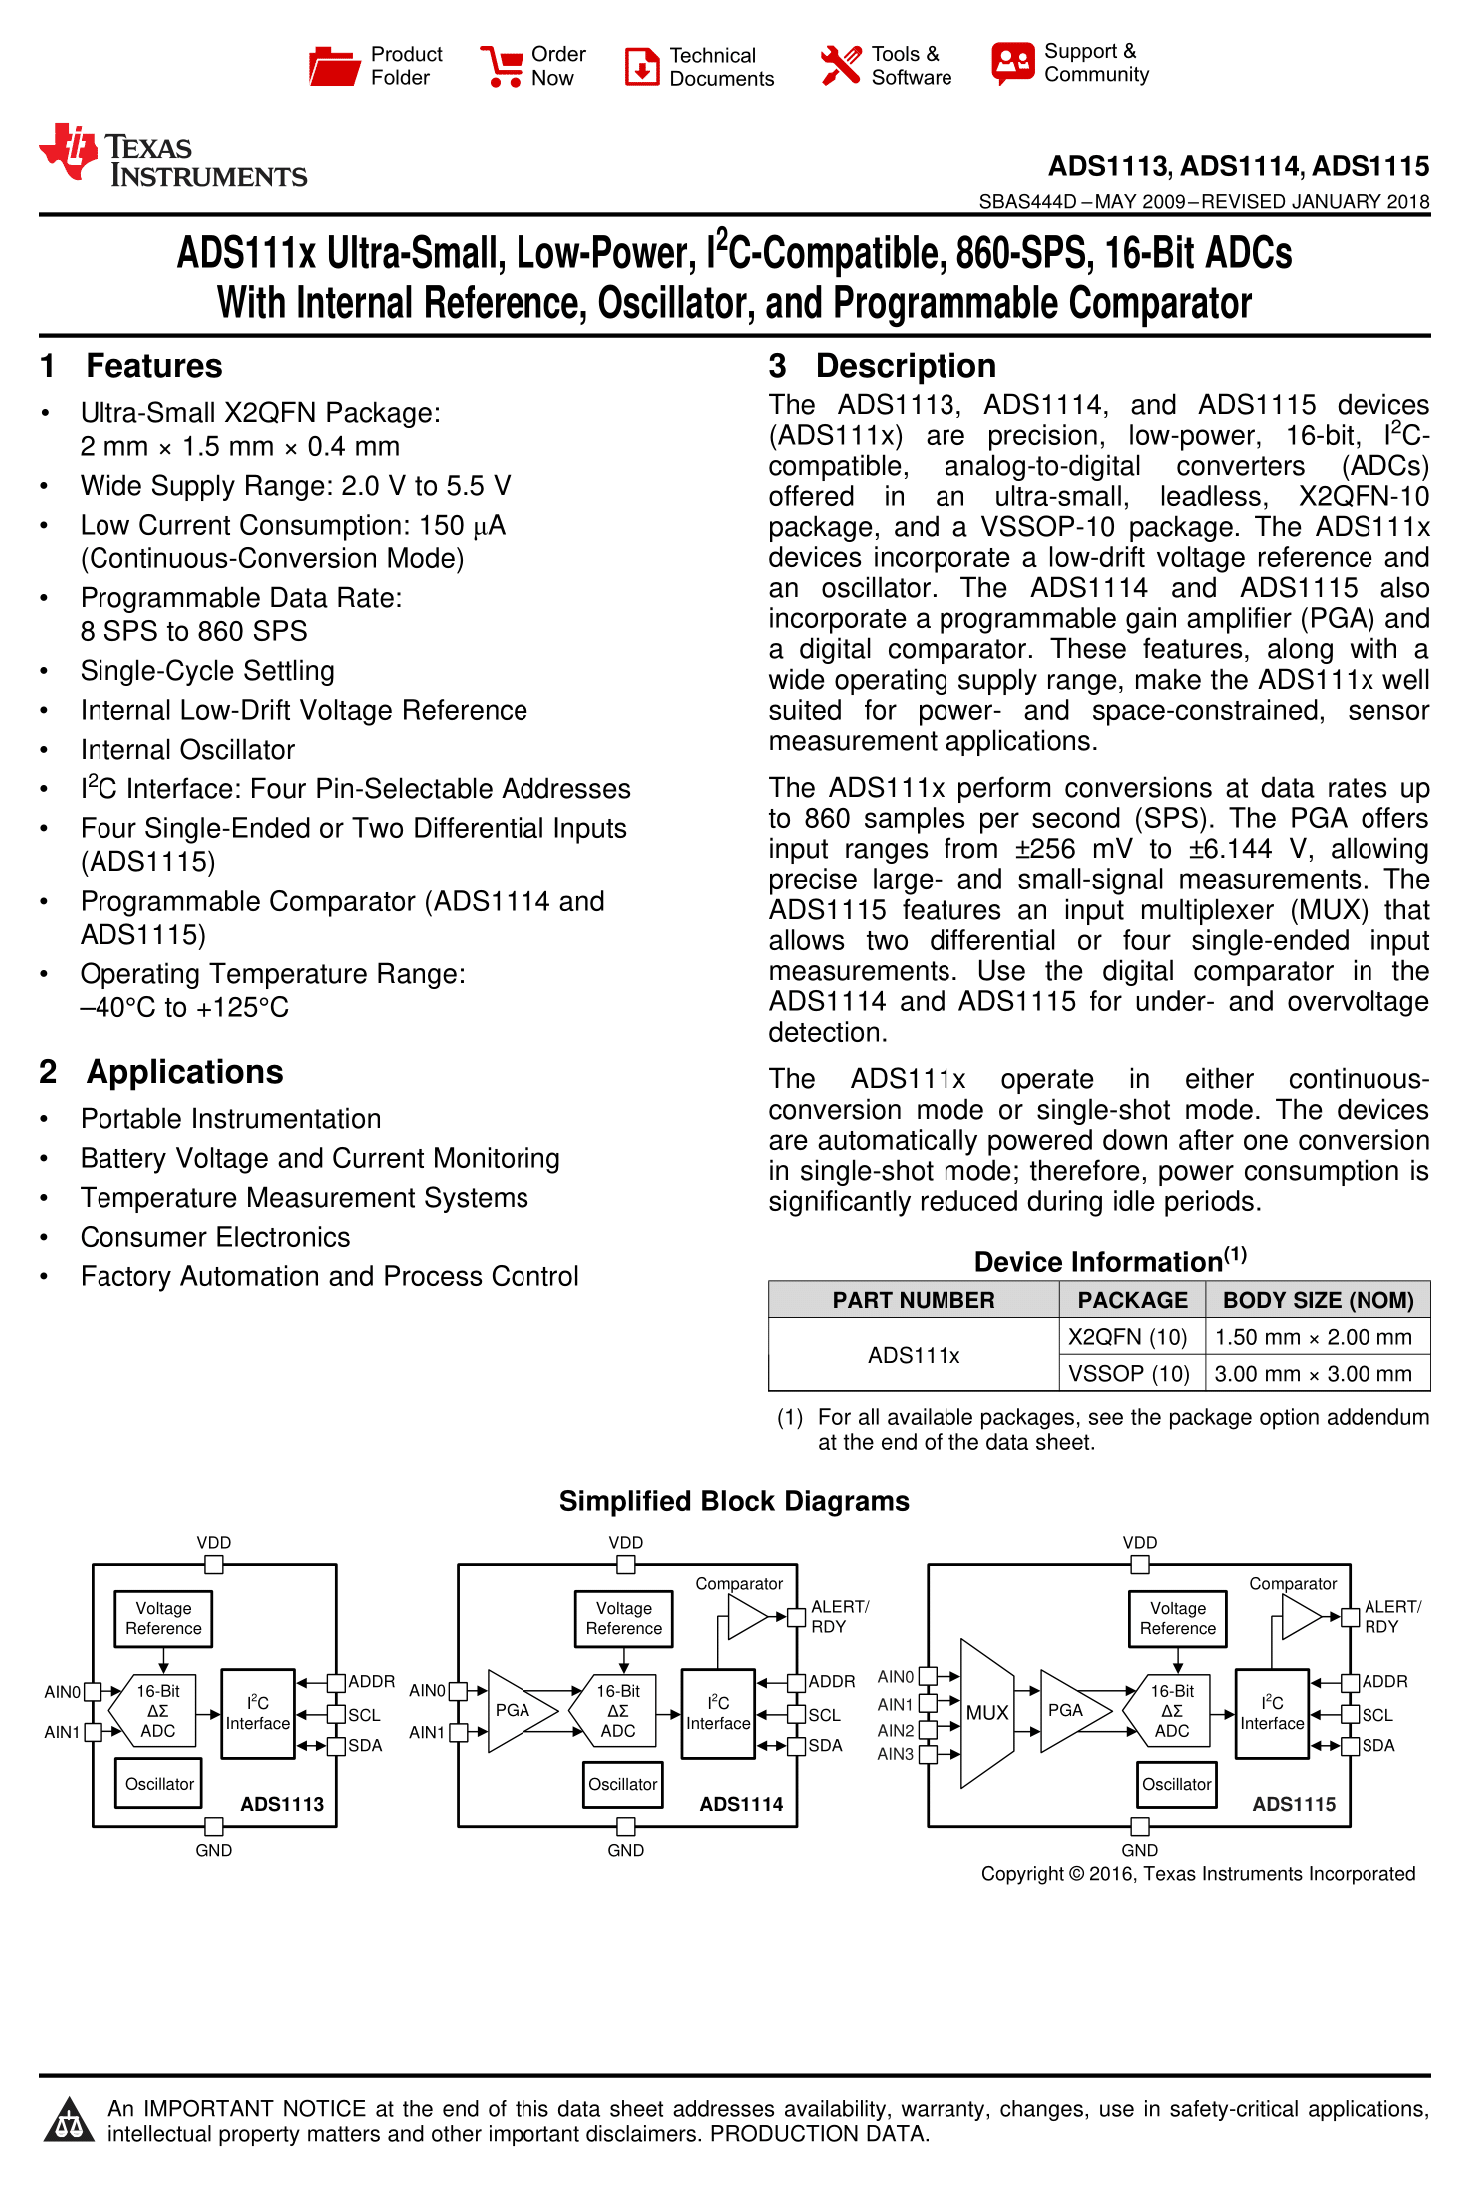
\includepdf[pages=-, scale=0.6]{Anexos/ads1115.pdf}
	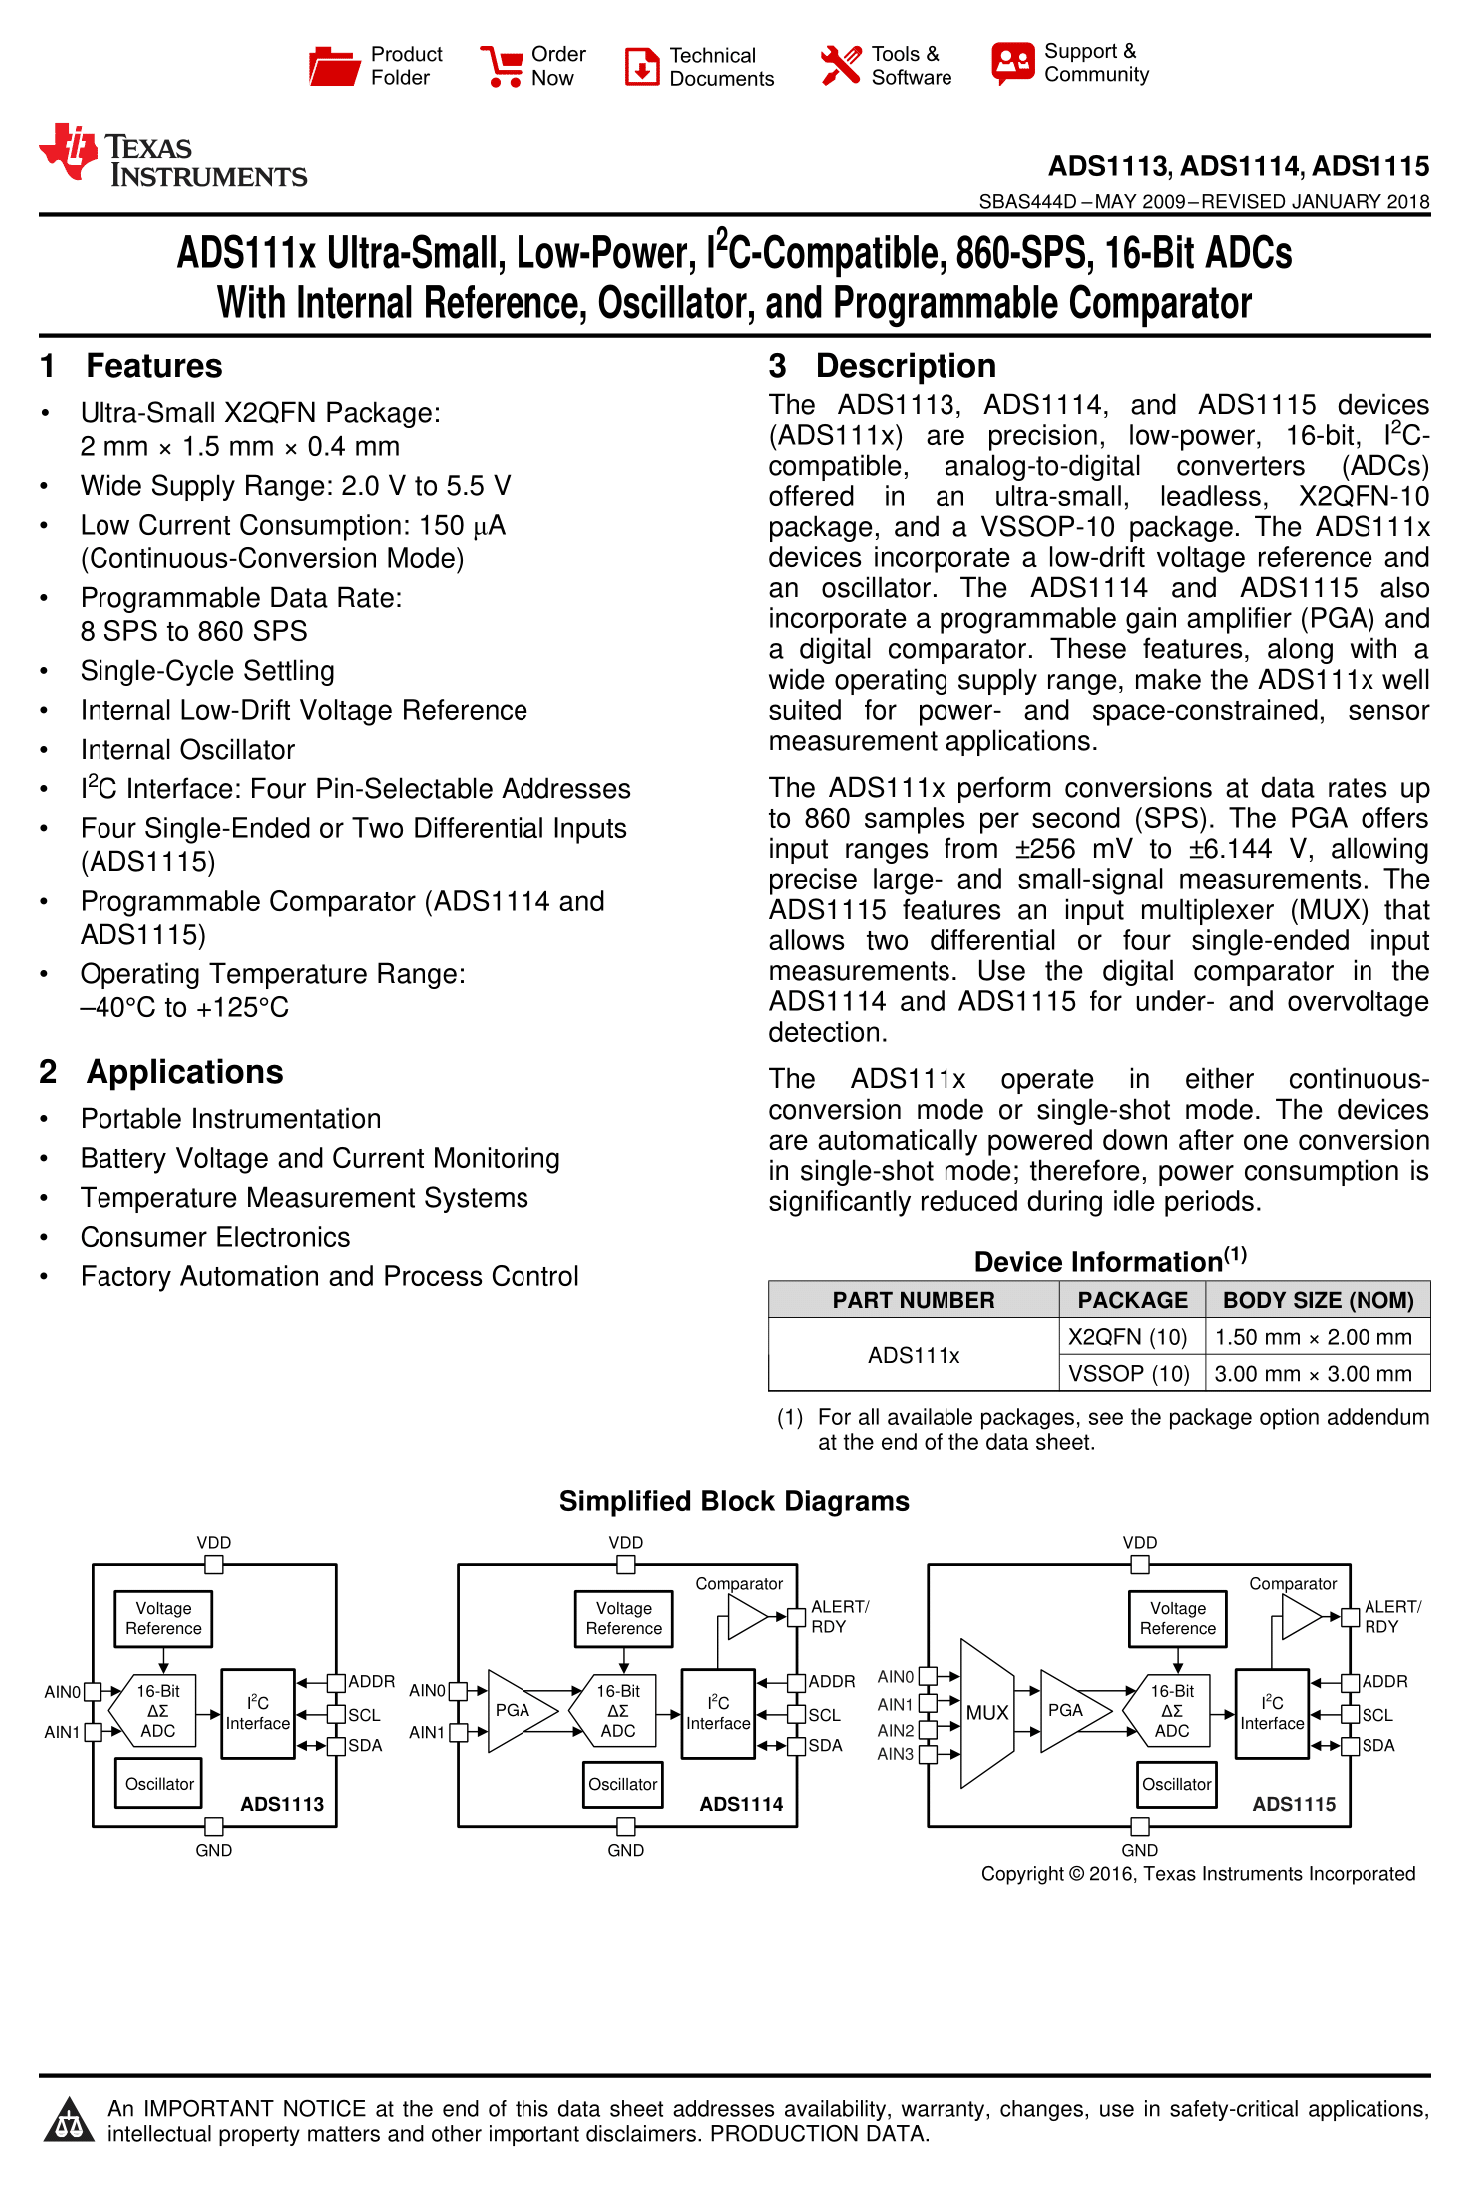
\includegraphics[scale=0.35]{Anexos/ads1115.png}
	
	\FloatBarrier
	Disponível em:\url{http://www.ti.com/lit/ds/symlink/ads1115.pdf}.
%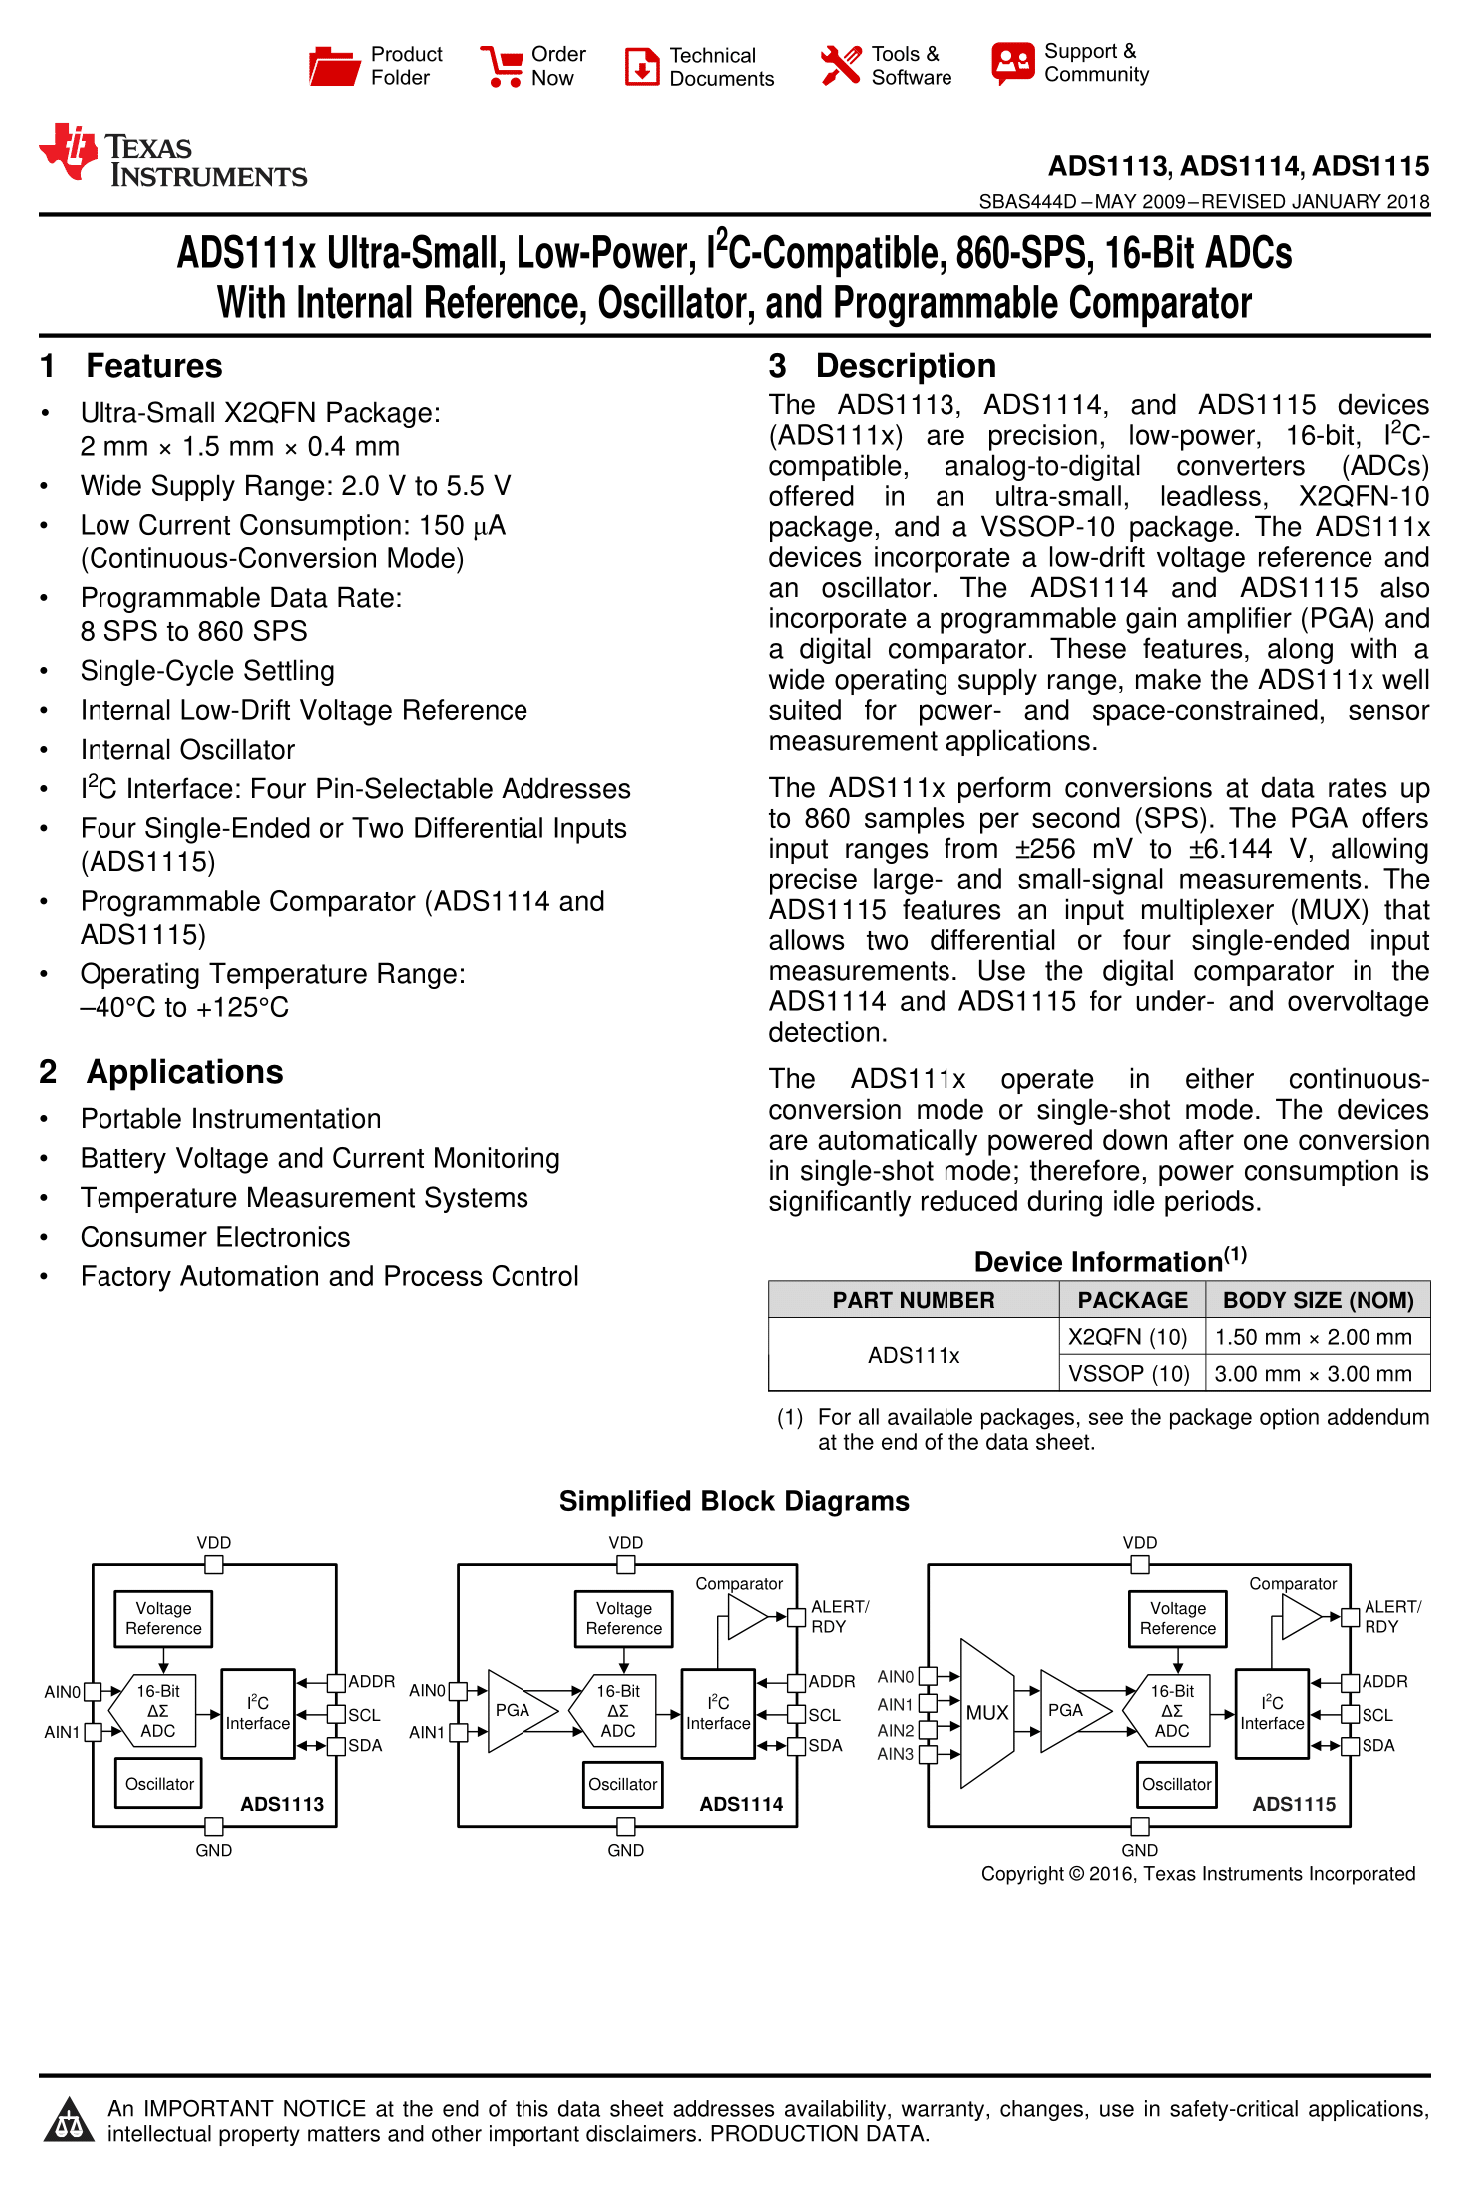
\includepdf[pages=-, scale=0.6, offset=75 -75]{Anexos/ads1115.pdf}

	
	% ----------------------------------------------------------
	\chapter{Título do Anexo B}
	% ----------------------------------------------------------
	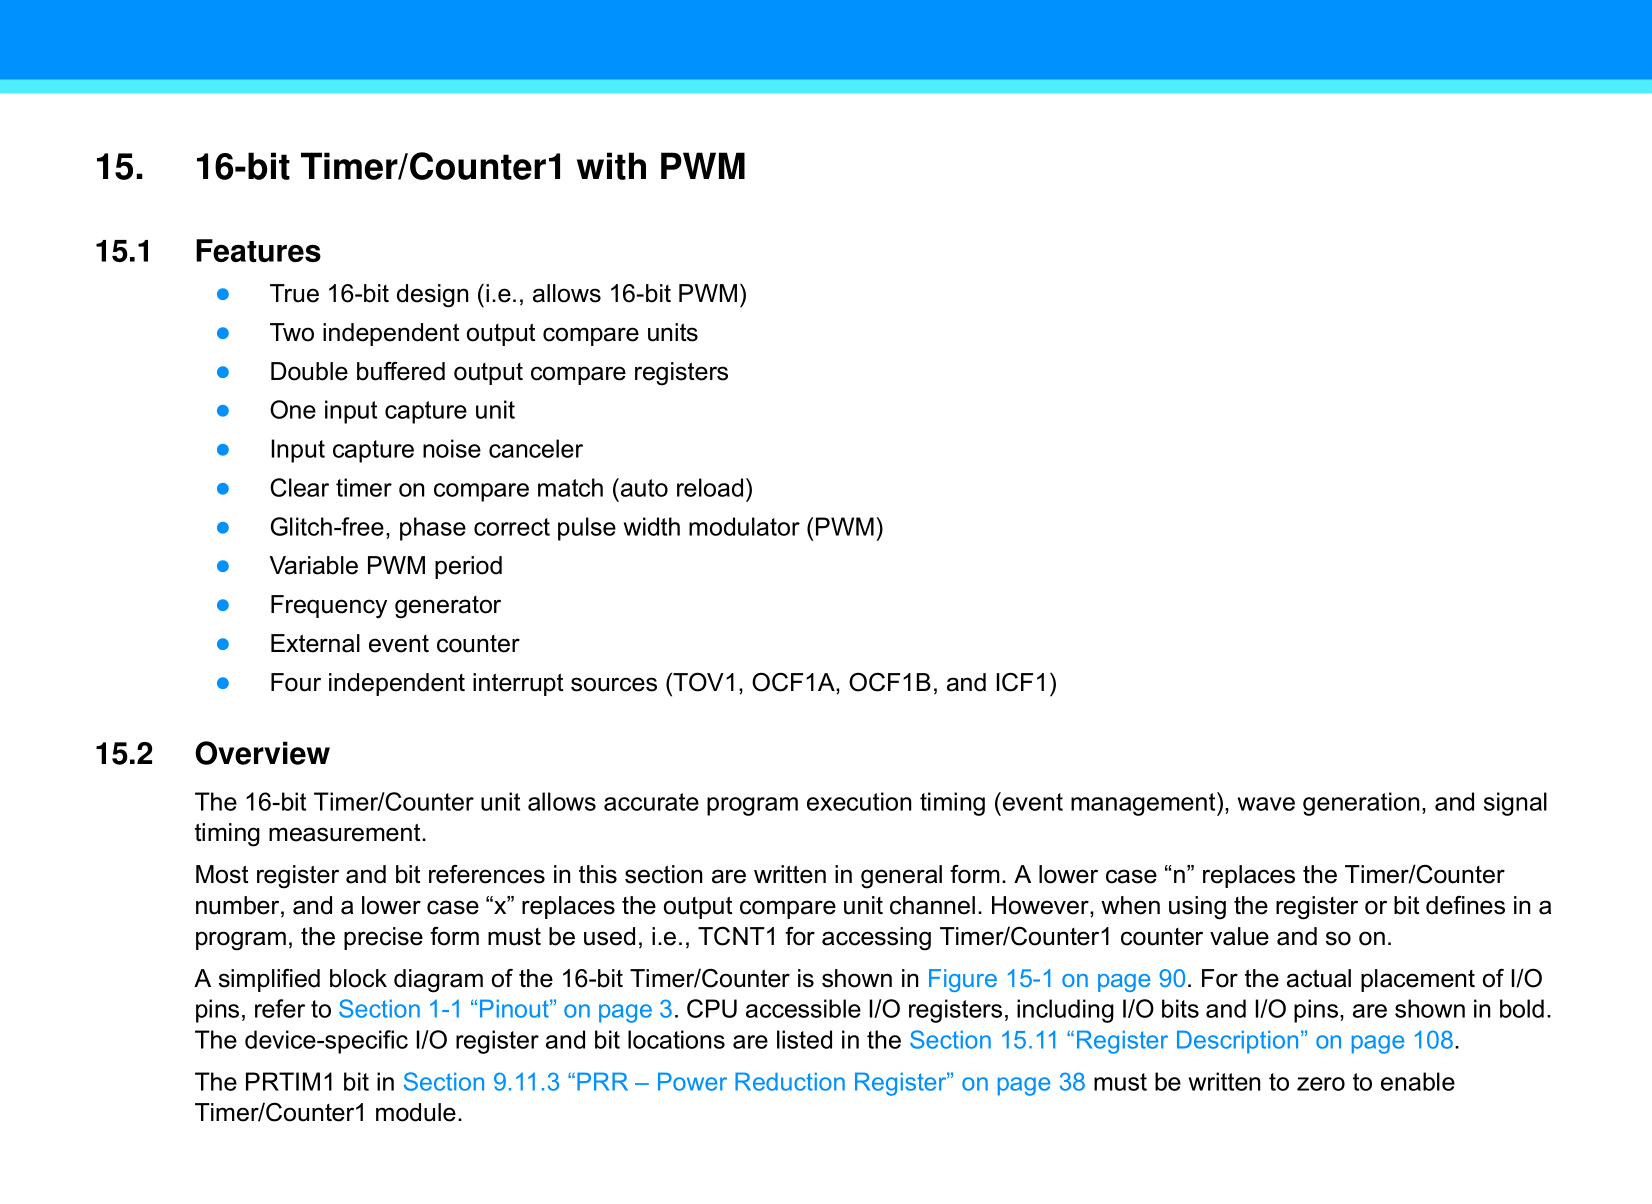
\includegraphics[scale=0.3]{Anexos/Atmel-089.png}
		\FloatBarrier
	Datasheet Atmega328p, Disponível em:\url{http://ww1.microchip.com/downloads/en/DeviceDoc/Atmel-7810-Automotive-Microcontrollers-ATmega328P_Datasheet.pdf}.

\end{anexosenv}